\section{Potenciais de medida conhecida}

Podemos validar a execução do programa e qualidade da medida gerada utilizando de potenciais bem descritos na literatura. Para isso, retomaremos os resultados da Seção \ref{Section: Potencias}. Foi comentado que modelos de matrizes aleatórias são úteis em simulações das medidas quando um modelo está disponível. A família de ensembles gaussianos são modelos que mostramos ser bem representados como matrizes em \ref{Section: Ensembles Gaussianos}. Tomar a medida dos ensembles gaussianos é o equivalente na simulação descrita a tomar 
\begin{equation}
d = 1, \ \  n = 2, \ \ \V(x)=\frac{|x|^2}{2}, \ \ W(x) = g(x) = \log{|x|}, \ \ \beta_N = \beta N^2, \ \ \beta = 1,2,4.
\label{Equation: Parametros Gaussian}
\end{equation}
O resultado da simulação para \ref{Equation: Parametros Gaussian} está na Figura \ref{Figura: Gaussian}. Apresentamos ainda na coluna da esquerda os resultados, para $N=10$, da densidade gerada pela simulação equivalente com matrizes para os três modelos ($\beta = 1,2,4$). Na coluna central, representa-se uma comparação com o Semi-Círculo de Wigner, configuração de equilíbrio para os três modelos quando $N$ é grande o suficiente. Note que os valores foram escalados por $\sqrt{2 \beta}$ para melhor visualização. Finalmente, na coluna da direita apresentamos a distribuição do maior autovalor. Um resultado importante  \cite{Tracy} enuncia que existem $z_{N}^{(\beta)}$ e $s_N^{(\beta)}$ tais que $$\lim_{N \to \infty} \mathbb{P}_{\beta,N,V} \left( \frac{\lambda_{max} - z_{N}^{(\beta)}}{s_N^{(\beta)}} \leq x \right) = F_{\beta}(x),$$ onde $F_{\beta}(x)$ é a densidade acumulada de Tracy-Widow. Mostraremos a concordância desse resultado com a simulação na coluna da direita.
\begin{figure}[ht!]
	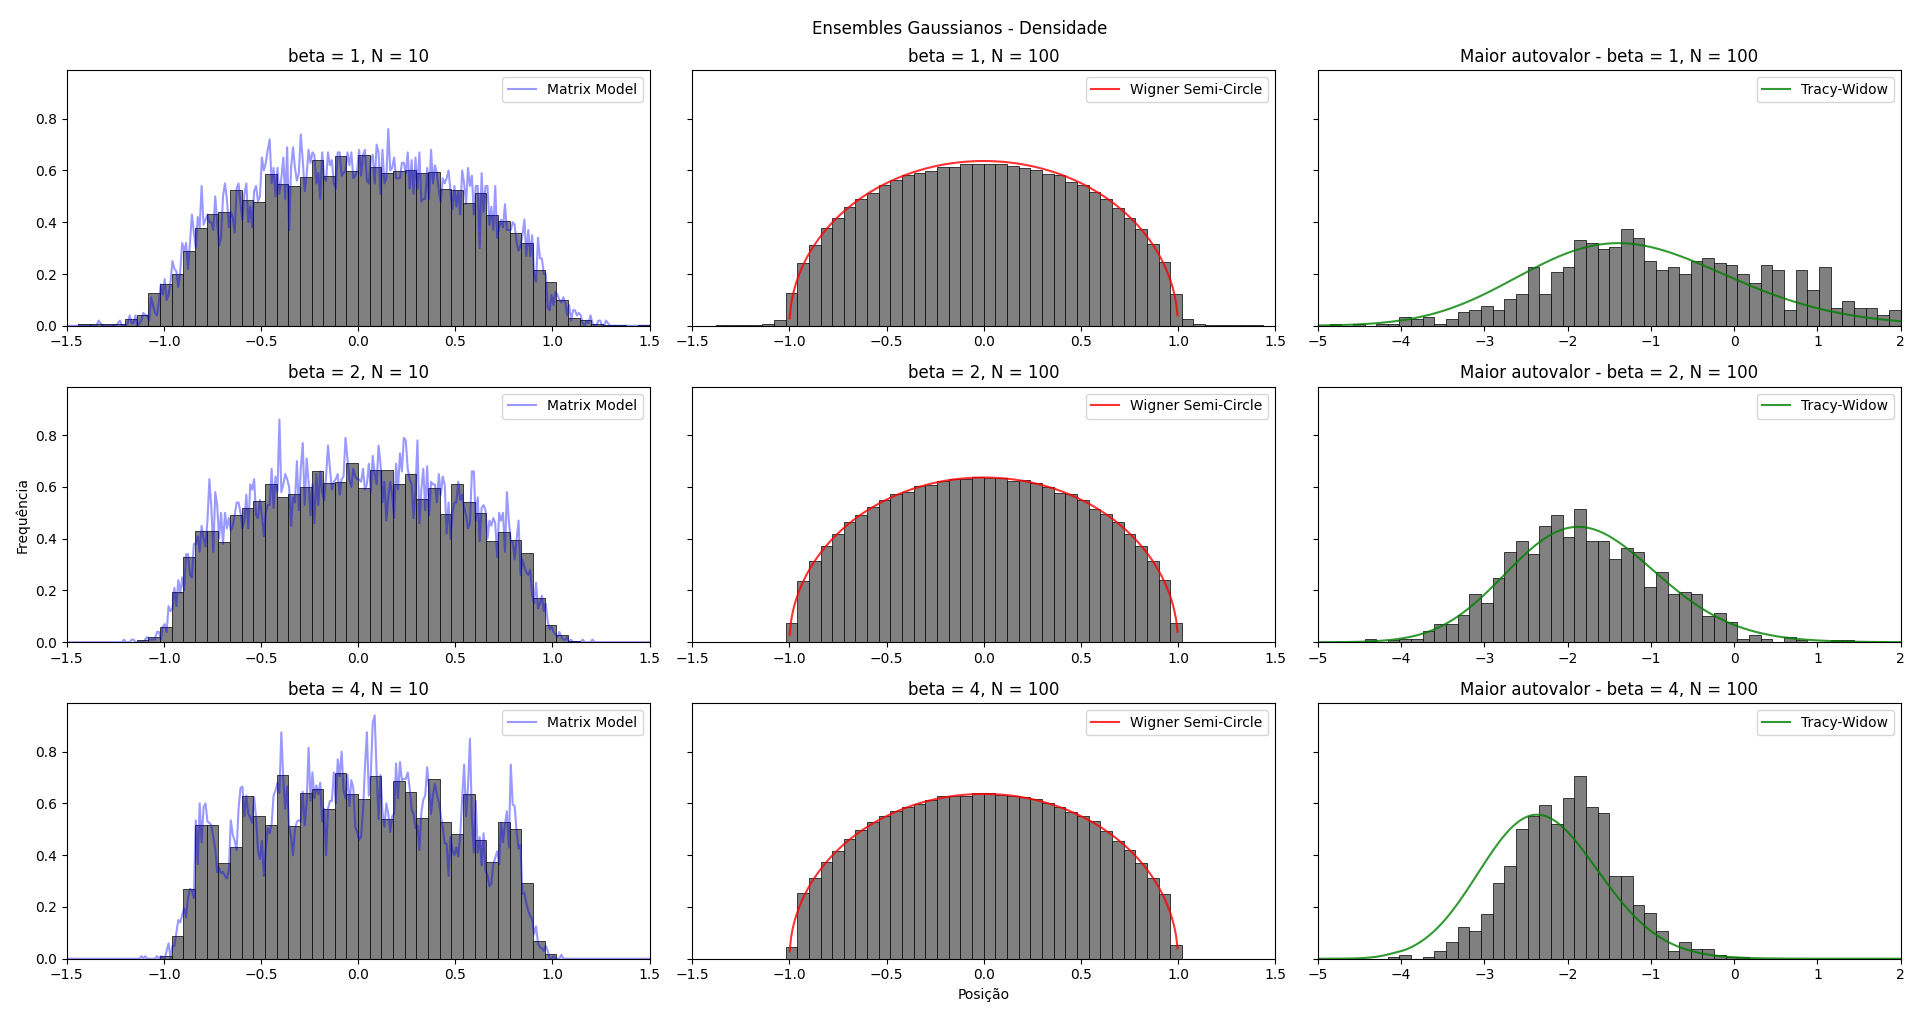
\includegraphics[width=\textwidth]{Assets/validationGaussianTracy.png}
	\caption{Densidade para ensembles gaussianos, \ref{Equation: Parametros Gaussian}. Tomou-se $\Delta t = 0.3$ e $nsteps = 5\cdot10^6$ passos, registrando a cada $1000$ iterações a partir de $nsteps/5$. À esquerda da figura, em azul, a densidade da amostragem de $4\cdot10^3$ matrizes do ensemble. No centro, o Semi-Círculo de Wigner, medida de equilíbrio. Na direita, apresenta-se a densidade de $\lambda_{max}$ normalizado e sua mediada esperada.}
	\label{Figura: Gaussian}
\end{figure}

Indo além dos modelos gaussianos podemos retomar as descrições dos potenciais mônico em \ref{Equação: Mônico} e as duas situações para o potencial quártico \ref{Equação: Quartico +} e \ref{Equação: Quartico -}. Respectivamente, estes modelos equivalem a tomar na simulação os parâmetros
\begin{equation}
	d = 1, \ \  n = 2, \ \ \V(x)= t |x|^{2m}, \ \ W(x) = g(x) = \log{|x|}, \ \ \beta_N = \beta N^2, \ \ \beta = 2.
	\label{Equation: Parametros Monico}
\end{equation}
\begin{equation}
	d = 1, \ \  n = 2, \ \ \V(x)=\frac{|x|^4}{4} + t \frac{|x|^2}{2}, \ \ W(x) = g(x) = \log{|x|}, \ \ \beta_N = \beta N^2, \ \ \beta = 2.
	\label{Equation: Parametros Quartico}
\end{equation}
O caso mônico se reduz ao gaussiano se $m=1$. Os resultados para ambos os potenciais estão explicitados na Figura \ref{Figura: Quartic Monic} para alguns parâmetros interessantes de $t$ e $m$.
\begin{figure}[ht!]
	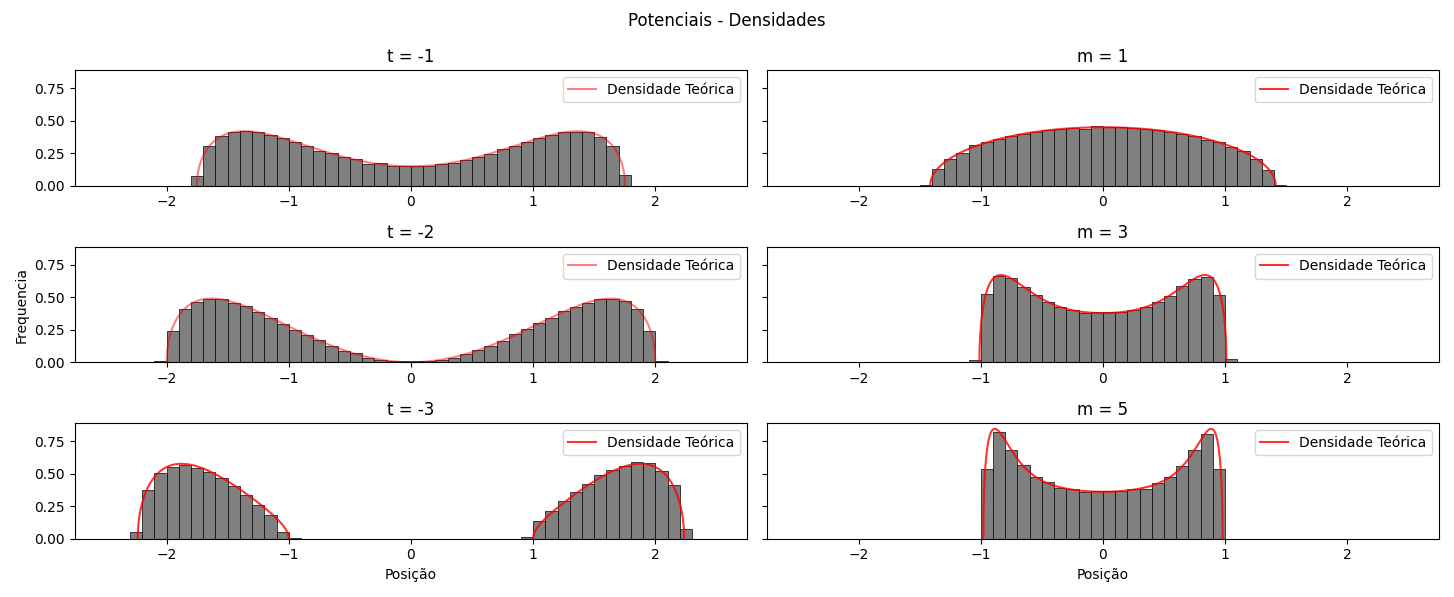
\includegraphics[width=\textwidth]{Assets/validationQuarticMonic-alt.png}
	\caption{Potencial Quártico \ref{Equation: Parametros Quartico} e Mônico \ref{Equation: Parametros Monico}, respectivamente à esquerda e direita. Tomou-se $\Delta t = 0.1$, $N=100$, e $nsteps = 5\cdot10^6$ passos. Registra-se a cada $1000$ iterações a partir de $nsteps/5$. No Quártico, simula-se $t=-1,-2,-3$. No Mônico fixa-se $t=1$ e simula-se $m=1,3,5$.}
	\label{Figura: Quartic Monic}
\end{figure}

